\chapter{Wellen in einem Kanal}
\label{chapter:wellen}
\lhead{Wellen in einem Kanal}
\begin{refsection}
\chapterauthor{Daniela Meier und Hansruedi Patzen}

\begin{equation}
	y'' + (ax^2+bx+c)y = 0
	\label{eq:wellen:grundgleichung}
\end{equation}

Dieses Kapitel besch"aftigt sich mit Ausbreitung von Wellen in einem 
parabolischen Kanal. Die Ausbreitung wird mittels Analyse der Wellengleichung 
n"aher betrachtet.

%
% einleitung.tex -- Einleitung zum Skript ueber Differentialgleichungen
%
% (c) 2015 Prof Dr Andreas Mueller, Hochschule Rapperswil
%
\chapter{Einleitung\label{chapter:einleitung}}
\lhead{Einleitung}
\rhead{}
In XKCD 135 (Abbildung~\ref{einleitung:xkcd135})
beschreibt Randall Munroe erdachte Aufgaben "uber die
Jagdgewohnheiten von Velociraptoren, Fragen, bei denen es um Leben
und Tod geht.
Die Aufgaben k"onnen zwar ohne Differentialgleichungen gel"ost
werden, aber sie k"onnen leicht zu noch spannenderen Aufgaben
verallgemeinert werden, die nicht ohne die Kenntnisse von 
Differentialgleichungen gel"ost werden k"onnen.
Dies zeigt, dass die Kenntnis der L"osungsverfahren von Differentialgleichungen
eine Frage von Leben und Tod ist.

\index{Newton!Isaac}
Isaac Newtons Grundgesetze der Dynamik sind die ersten Beispiele
von Differentialgleichungen.
Sein erstes Gesetz besagt:
\begin{quote}
\em
Ein K"orper verharrt im Zustand der Ruhe oder der gleichf"ormigen Translation,
sofern er nicht durch einwirkende Kr"afte zur "Anderung seines Zustands
gezwungen wird.
\end{quote}
In der Abwesenheit von Kr"aften ver"andert sich die Geschwindigkeit nicht,
oder 
\[
\frac{d}{dt}\vec{v}=0,
\]
wobei $\vec{v}$ der Vektor der Geschwindigkeit ist.
Das erste Gesetz oder Tr"agheitsprinzip wurde schon von Galileo Galilei
formuliert.
\index{Tragheitsprinzip@Tr\"agheitsprinzip}

\begin{figure}
\centering
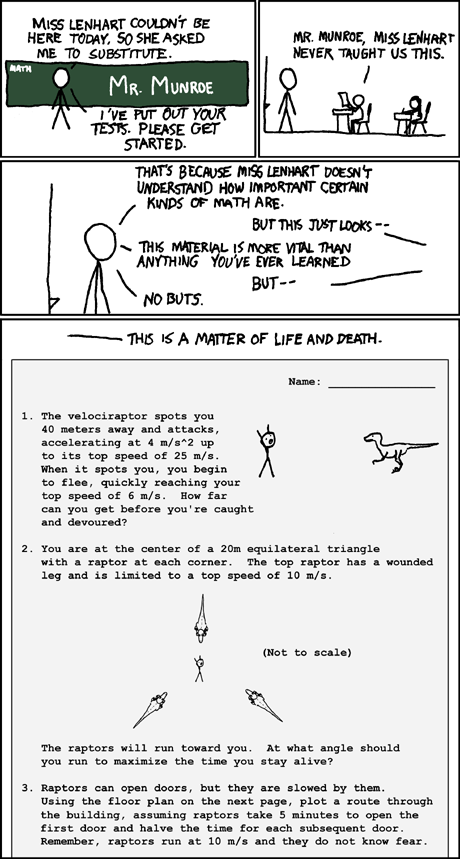
\includegraphics[width=0.7\hsize]{chapters/substitute.png}
\caption{xkcd 135 mit von Randall Munroe erdachten Aufgaben "uber die
Jagdgewohnheiten von Velociraptoren.
\label{einleitung:xkcd135}}
\end{figure}%


Das zweite Gesetz besagt:
\begin{quote}
\em
Die "Anderung der Bewegung ist der Einwirkung der bewegenden Kraft
proportional und geschieht nach der Richtung derjenigen geraden Linie,
nach welcher jene Kraft wirkt.
\end{quote}
Mit {\em Bewegung}
meint Newton den Impuls $\vec{p}=m\vec{v}$,
\index{Impuls}
das zweite Gesetz wird in moderner Schreibweise
\[
\frac{d}{dt}(m\vec{v}) = \vec{F}.
\]
In beiden F"allen wird die "Anderung einer Zustandsvariablen, n"amlich
des Impulses, mit dem aktuellen Zustand, typischerweise der Position,
verkn"upft.
Die Newtonsch-Bewegungsgesetze sind Differentialgleichungen.
\index{Newton!Bewegungsgesetz}

Das neue Werkzeug der Infinitesimalrechnung bescherte der exakten
Naturwissenschaft eine F"ulle neuer Probleml"osungen, die alle
nach dem gleichen Prinzip vorgingen.
Finde die Differentialgleichungen zwischen den Zustandsvariablen
eines Systems, "ublicherweise durch Anwendung des zweiten
Newtonschen Gesetztes, l"ose die Differentialgleichungen und
ziehe die Schl"usse.
Es zeigte sich jedoch bald, dass viele Differentialgleichungen
keine L"osungen haben, die sich mit den bisher bekannten Funktionen
ausdr"ucken lassen.
Man behalf sich kurzerhand damit, neue Funktionen zu definieren, 
die bald Anwendungen in den verschieden Gebieten der Technik fanden.
Die Bessel-Funktionen sind mittlerweile so wichtig, dass sie in keiner
Computer-Bibliothek f"ur mathematische Funktionen fehlen d"urfen.
\index{Bessel-Funktion}

Die Herkunft der Kr"afte wird in den Newtonschen Gesetzen nicht weiter
gekl"art, doch Newton selbst beschreibt mit seinem Gravitationsgesetz
die Herkunft der Kr"afte, die die Planeten im Sonnensystem auf ihren Bahnen
halten.
\index{Kepler!Johannes}
\index{Kepler-Bahn}
Er zeigt, dass die Keplerschen Ellipsenbahnen L"osungen seiner
Bewegungsgleichungen sind.
Die rein kinematische Beschreibung durch Kepler machte einem
dynamischen Verst"andnis Platz, welches nun auch die gegenseitigen
Einfl"usse der Planeten aufeinander zu berechnen gestattet.
Und tats"achlich war Newton der erste, der sich dar"uber Gedanken
machte, wie sich das Sonnensystem "uber lange Zeit entwickeln wird.
Seine Schlussfolgerung aus seinen aus heutiger Sicht rudiment"aren
Untersuchungen: das Sonnensystem ist instabil, "uber die Jahrmillionen 
werden die Planeten in den interstellaren Raum geschleudert werden.

Die industrielle Revolution brachte eine Vielzahl von Maschinen,
\index{industrielle Revolution}
die automatisch geregelt werden mussten.
Ingenieure entwickelten eine ganze Reihe von einfallsreichen L"osungen,
doch erst in der Mitte des 19.~Jahrhunderts konnten Physiker diese
Apparaturen mit Differentialgleichungen erkl"aren und ihre Stabilit"at
untersuchen.
Im zwanzigsten Jahrhundert reiften die mathematischen Hilfsmittel
soweit, dass auch instabile L"osungen untersucht werden konnten,
wie sie bei nichtlinearen Differentialgleichungen auftreten.
Mittlerweile ist das Auftreten Instabilit"aten recht gut verstanden
und klassifiziert. 
Die Technik der Linearisierung erm"oglicht zum Beispiel die
Hopf-Bifurkation zu verstehen.
\index{Hopf-Bifurkation}
\index{Bifurkation!Hopf}
Auch die Sattel-Knoten-Bifurkation und die Heugabel-Bifurkation
lassen sich in Anwendungen finden.
\index{Bifurkation!Sattel-Knoten-}
\index{Sattel-Knoten-Bifurkation}
\index{Bifurkation!Heugabel-}
\index{Heugabel-Bifurkation}
Und die Chaos-Theorie versteht sogar, wie "uber eine Kaskade von
Bifurkationen die Bewegung eines Systems jede Vorhersagbarkeit verliert,
es bewegt sich chaotisch.
\index{Chaos}

In vielen F"allen l"asst sich eine Differentialgleichung erst dann
verstehen, wenn man in komplexen Zahlen arbeiten. 
Die Hopf-Bifurkation tritt zum Beispiel genau dann auf, wenn eine
Bedingung "uber die Eigenwerte des linearisierten Systems erf"ullt ist.

Weitere Literaturhinweise im Literaturverzeichnis auf
Seite~\pageref{skript:literatur}.



\section{Herleitung Ausgangsformel}
Gem"ass \cite{wellen:smirnow2}, lautet die allgemeine Differentialgleichung der 
Welle:

\begin{equation*}
	\frac{\partial^2 u}{\partial t^2}
	=
	c^2
	\left(
		\frac{\partial^2 u}{\partial x^2} 
		+ \frac{\partial^2 u}{\partial y^2} 
		+ \frac{\partial^2 u}{\partial z^2}
	\right)
	\label{eq:wellen:allgemeineDGL}
\end{equation*}

Da es sich in der ausgew"ahlten Problemstellung nur eine zweidimensionale Welle 
handelt, fallen die y- und z-Koordinate weg. Die Gleichung vereinfacht sich 
dadurch zu:

\begin{equation}
	\frac{\partial^2 u}{\partial t^2}
	=
	c^2
	\left(
		\frac{\partial^2 u}{\partial x^2} 
	\right)
	\label{eq:wellen:allgemeineDGLvereinfacht}
\end{equation}

Zur L"osung der vereinfachten Wellengleichung 
\ref{eq:wellen:allgemeineDGLvereinfacht} wird nun die Theorie des 
Separationsansatzes angewendet. Gem"ass dieser kann die von der Zeit $t$ und 
der Ortskoordinate $x$ abh"angigen Funktion $u(x,t)$ in ein Produkt 
zweier Funktionen $X(x)$ und $T(t)$ umgewandelt werden.

\begin{equation}
	u (x,t) = X(x) T(t)
	\label{eq:wellen:separierteFunktion}
\end{equation}

Ausgehend von der Gleichung \ref{eq:wellen:allgemeineDGLvereinfacht} wird die 
Funktion \ref{eq:wellen:separierteFunktion} auf der linken Seite zweimal 
partiell nach $t$ und auf der rechten Seite zweimal partiell nach $x$ 
abgeleitet:

\begin{equation*}
	T''(t) X(x) = c^2 X''(x)T(t)
\end{equation*}

Nach einer Division durch $T(x)X(x)$ sind die Variablen separiert. Der neu 
entstandene Term kann nur dann funktionieren, wenn beide Seiten der Gleichung 
konstant sind.

\begin{equation*}
	\frac{T''(t)}{T(t)}
	=
	c^2 \frac{X''(x)}{X(x)} = \text{konstant} = \lambda
\end{equation*}

Es folgen nun also zwei l"osbare Differentialgleichungen zweiter Ordnung:

\begin{align*}
	T'' &= \lambda T(t) \\
	X'' &= \frac{\lambda}{c^2}X(x).
\end{align*}

Bei der betrachteten Problemstellung, wird davon ausgegangen, dass die 
Zeit konstant ist. Aus diesem Grund wird ab hier nur noch auf die Gleichung 
der Funktion $X(x)$ weiter eingegangen.

Die Gleichung

\begin{equation*}
	X''(x) - \frac{\lambda}{c^2} X(x) = 0
\end{equation*}
widerspiegelt die Wellengleichung, die in der Fortsetzung betrachtet wird.

Mit dem Faktor $\frac{\lambda}{c^2}$ k"onnen verschiedene 
Geschwindigkeitsprofile betrachtet werden. Hier wird unter anderem auf den 
speziellen Fall eines parabolischen Profils eingegangen. Die zu untersuchende 
Differentialgleichung ergibt sich hiermit zu der am Anfang definierten 
Gleichung \ref{eq:wellen:grundgleichung}, mit den frei w"ahlbaren Variablen 
${a,b,c} \in \mathbb{R}$, sowie den Anfangsbedingungen $y(0) = a_0$ und $y'(0) 
= a_1$.


\section{Potenzreihenl"osung}
Als L"osungsansatz wird der im Kapitel \ref{chapter:potenzreihen} 
kennengelernte Potenzreihenansatz verwendet.

Zuerst wird die Potenzreihe f"ur $y(x)$ aufgestellt und zweimal abgeleitet.

\begin{align}
	y(x)
	&=
	\sum_{k = 0}^{\infty} a_{k}x^k
	=
	a_0 + a_1x + a_2x^2 + a_3x^3 + a_4x^4 + a_5x^5 + a_6x^6 + \dotsb
	\label{eq:wellen:nullteableitung}
	\\
	y'(x)
	&=
	\sum_{k=0}^{\infty} a_{k+1}(k+1)x^k
	=
	a_1 + 2a_2x + 3a_3x^2 + 4a_4x^3 + 5a_5x^4 + 6a_6x^5+ \dotsb
	\label{eq:wellen:ersteableitung}
	\\
	y''(x)
	&=
	\sum_{k = 0}^{\infty} a_{k+2}(k+1)(k+2)x^k
	=
	2a_2 + 3 \mathbin{\cdot} 2a_3x + 4 \mathbin{\cdot} 3a_4x^2 + 5 
	\mathbin{\cdot} 4a_5x^3 + 6 \mathbin{\cdot} 5a_6x^4 + \dotsb
	\label{eq:wellen:zweiteableitung}
\end{align}

Aus den beiden Gleichungen \ref{eq:wellen:nullteableitung} und
\ref{eq:wellen:zweiteableitung} und dem Umstellen der Anfangsgleichung in die 
Form
\begin{equation*}
	y'' = -(ax^2+bx+c)y
\end{equation*}
kann nun der Koeffizientenvergleich erstellt werden. 

Statt die Koeffizienten einfach reihenweise aufzustellen, wird der Vergleich 
mit Hilfe einer Tabelle gemacht.

\begin{equation}
	\begin{array}{r c r | c r | c r | c r c}
	y(x) & = &
	a_0 & + & a_1x & + & a_2x^2 & + \dotsb
	\\
	\hline&&&&&&&\\[-2ex]
	y''(x) & = &
	2\cdot1 a_2 & + & 3\cdot2 a_3x & + & 4\cdot3 a_4x^2 & + \dotsb
	\\
	& = &
	& & & + &- aa_0x^2 & + \dotsb
	\\
	& &
	& &- ba_0x & + &- ba_1x^2 & + \dotsb
	\\
	& &
	-ca_0 & + &- ca_1x & + &- ca_2x^2 & + \dotsb
	\\
	\hline&&&&&&&\\[-2ex]
	& &
	a_2 = -\frac{1}{2 \cdot 1}ca_0,
	& & a_3 = -\frac{1}{3 \cdot 2}(ba_0+c_a1),
	& & a_4 = -\frac{1}{4 \cdot 3}(aa_0+ba_1+ca_2),
	& \dots
	\end{array}
	\label{eq:wellen:koeffizietenvergleichtabelle}
\end{equation}

Die Verschiebung der verschiedenen $a_k$ in der Tabelle 
\ref{eq:wellen:koeffizietenvergleichtabelle} kann einfach erkl"art werden. 
Aufgrund der zweiten Ableitung werden die $a_k$ der zweiten Zeile um zwei nach 
links geschoben. Eine weitere Verschiebung gibt es wegen des Polynomgrades.

Da die $a$-Summanden mindestens die Form $ax^2$ haben, verschiebt sich die 
dritte Zeile um zwei nach rechts. Die $b$-Summanden haben mindestens Die Form 
$bx^1$, daher die Verschiebung der vierten Zeile um eins nach rechts. Einzig 
die f"unfte Zeile mit den $c$ wird nicht verschoben, da es mindestens als 
$cx^0$ vorhanden ist. Somit lassen sich die jeweiligen $a_k$ und ihre 
Abh"angigkeiten direkt aus den jeweiligen Spalten ablesen.

Aus den in der Tabelle berechneten $a_k$ l"asst sich nun eine allgemeine 
Rekursionsformel

\begin{equation*}
	\begin{split}
		a_{k+2} &= -\frac{1}{(k+2)(k+1)} (aa_{k-2}+ba_{k-1}+ca_k) \\
		\Leftrightarrow \qquad
		a_k &= -\frac{1}{k(k-1)} (aa_{k-4}+ba_{k-3}+ca_{k-2}), \qquad k \in 
		\mathbb{N} \setminus \{0, 1\}, a_{k<0} = 0
	\end{split}
\end{equation*}
herauslesen. 

Daraus kann nun die L"osungsgleichung
\begin{equation}
	y(x) = a_0 + a_1x 
	-\sum_{k=2}^{\infty}\frac{1}{k(k-1)}(aa_{k-4}+ba_{k-3}+ca_{k-2})x^k
	\label{eq:wellen:ygleichung}
\end{equation}
aufgestellt werden.


\section{Parametervariation}
\label{sec:wellen:parametervariation}

Die Anfangsbedingungen $a_0$ und $a_1$ k"onnen beliebig festgelegt werden. Da 
sich die Wellen im betrachteten Fall um den Entwicklungspunkt $x_0=0$ bewegen, 
beschreibt das $a_0$ den y-Achsenabschnitt und das $a_1$ die Steigung im Punkt 
$y(0)$.

\subsection{Bedeutung von \texorpdfstring{$a$}{a}, \texorpdfstring{$b$}{b} und 
\texorpdfstring{$c$}{c}}
Die drei Parameter $a$, $b$ und $c$ haben jeweils unterschiedliche Auswirkungen 
auf die Parabel. So kann mit $a$ der Schnittpunkt mit der $x$-Achse und mit $c$ 
derjenige mit der $y$-Achse festgelegt werden. $b$ hingegen verschiebt die 
ganze Parabel in verschiedene Richtungen. Da diese Eigenschaft f"ur das 
gegebene Modell nicht relevant ist, wird grunds"atzlich
\begin{equation*}
	b = 0
\end{equation*}
gesetzt.

\subsection{Lineare Differentialgleichung}
\label{subsec:wellen:linearedifferntialgleichung}

Indem $a$ verschwindend klein gew"ahlt wird, entsteht
\begin{equation}
	y''+ cy = 0.
	\label{eq:wellen:lineareDGL}
\end{equation}

Diese lineare Differentialgleichung kann mit Hilfe des charakteristischen 
Polynoms
\begin{equation*}
	p(\lambda) = [(\lambda+\mu)^2+\omega^2] = 0
\end{equation*}
dessen L"osungen
\begin{equation*}
\begin{split}
	y_1 &= C_1e^{-\mu x}\cos(\omega x) \\
	y_2 &= C_2e^{-\mu x}\sin(\omega x)
\end{split}
\end{equation*}
sind, gel"ost werden.

Angewandt auf die Gleichung \ref{eq:wellen:lineareDGL} ergibt sich nun zu
\begin{equation*}
\begin{split}
	p(\lambda) &= [(\lambda+0)^2+\sqrt{c}^2] = 0 \\
	\Leftrightarrow p(\lambda) &= [\lambda^2+c] = 0,
\end{split}
\end{equation*}
was uns nun
\begin{equation}
y(x) = C_1 \cos(\sqrt{c}x) + C_2 \sin(\sqrt{c}x)
\label{eq:wellen:loesunglinearedgl}
\end{equation}
als L"osung ergibt.

Um die Konstanten $C_1$ und $C_2$ zu bestimmen m"ussen die Anfangsbedingungen 
$a_0$ und $a_1$ bekannt sein. Damit die Abh"angigkeit auf gezeigt werden kann, 
wird zuerst die erste Ableitung der L"osung \ref{eq:wellen:loesunglinearedgl} 
aufgestellt werden.

\begin{equation}
	y'(x)=-C_1 \sqrt{c} \sin(\sqrt{c}x) + C_2 \sqrt{c} \cos(\sqrt{c}x)
\end{equation}

Die werte von $y(0)$ und $y'(0)$ sind jeweils durch $a_0$ beziehungsweise $a_1$ 
gegeben. Setzt man nun $x = 0$ ein, ergibt sich f"ur $C_1$ und $C_2$
\begin{equation}
	\begin{split}
		y(0) = C_1 = a_0 &\Leftrightarrow C_1 = a_0 \\
		y'(0) = C_2 \sqrt{c} = a_1 &\Leftrightarrow C_2 = \frac{a_1}{\sqrt{c}}.
	\end{split}
\end{equation}

Eingesetzt in \ref{eq:wellen:loesunglinearedgl} erhalten wir nun
\begin{equation*}
	y(x) = a_0 \cos(\sqrt{c}x) + \frac{a_1}{\sqrt{c}} \sin(\sqrt{c}x), \qquad c 
	> 0
\end{equation*}
und
\begin{equation}
\begin{split}
	y(x) &= a_0 \cos(i\sqrt{|c|}x) + \frac{a_1}{i\sqrt{|c|}}\sin(i\sqrt{|c|}x), 
	\qquad c < 0\\
	\Leftrightarrow
	y(x) &= a_0 \cos(i\sqrt{|c|}x) - i\frac{a_1}{\sqrt{|c|}}\sin(i\sqrt{|c|}x)\\
	\Leftrightarrow
	y(x) &= a_0 \cosh(\sqrt{|c|}x) + \frac{a_1}{\sqrt{|c|}}\sinh(\sqrt{|c|}x).
\end{split}	
\end{equation}
Der letzte Umformungsschritt ergibt sich aus der Definition von $\cosh$ und 
$\sinh$:
\begin{equation*}
\begin{split}
	\sinh(x) &= \frac{1}{2} (e^x - e^{-x}) = -i \sin(ix)\\
	\cosh(x) &= \frac{1}{2} (e^x + e^{-x}) = \cos (ix)
\end{split}
\end{equation*}

Die gefundenen L"osungen k"onnen auch graphisch best"atigt werden. Sei es f"ur 
positve $c$ in Form von $\sin$ und $\cos$:

\noindent
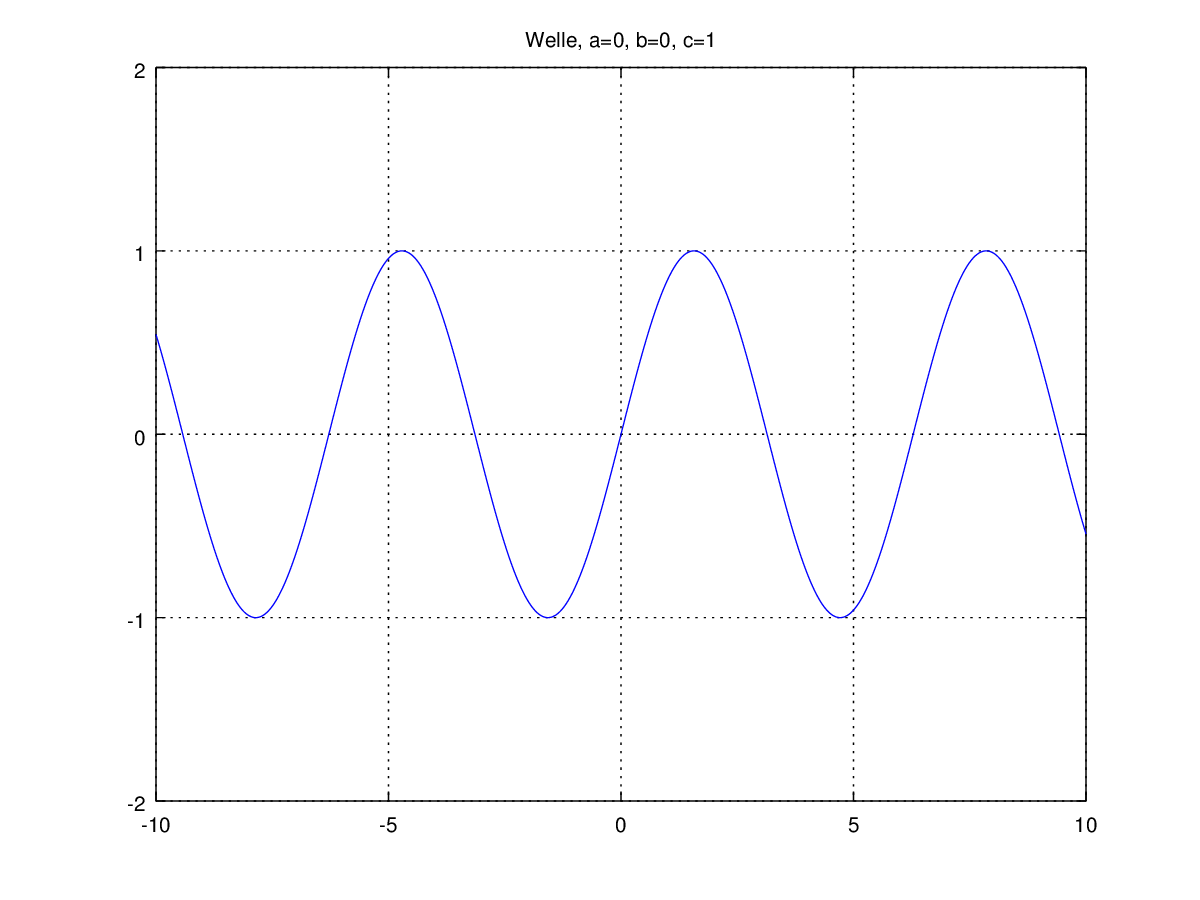
\includegraphics[scale=0.35]{./wellen/images/basicfunctions/sin.png}
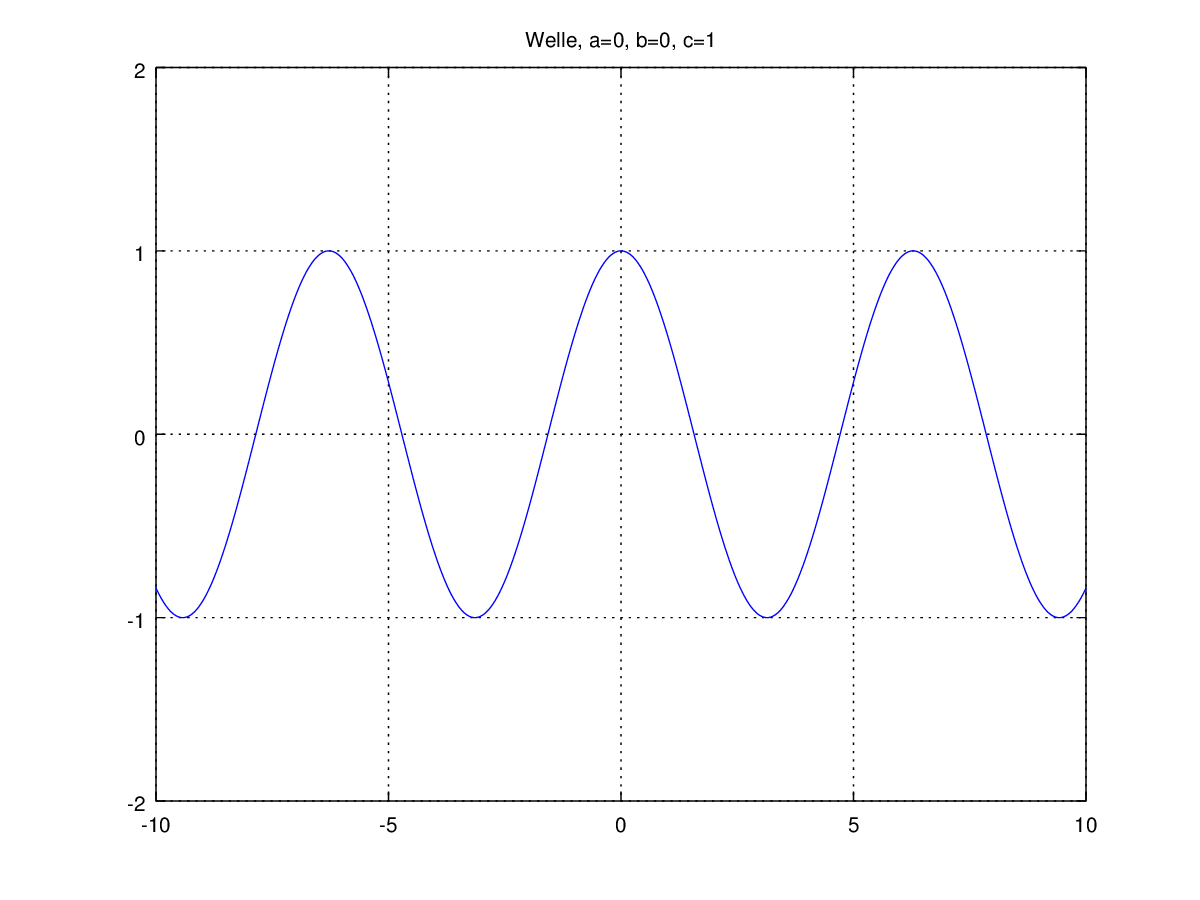
\includegraphics[scale=0.35]{./wellen/images/basicfunctions/cos.png}

oder $\sinh$ und $\cosh$ f"ur negative $c$:

\noindent
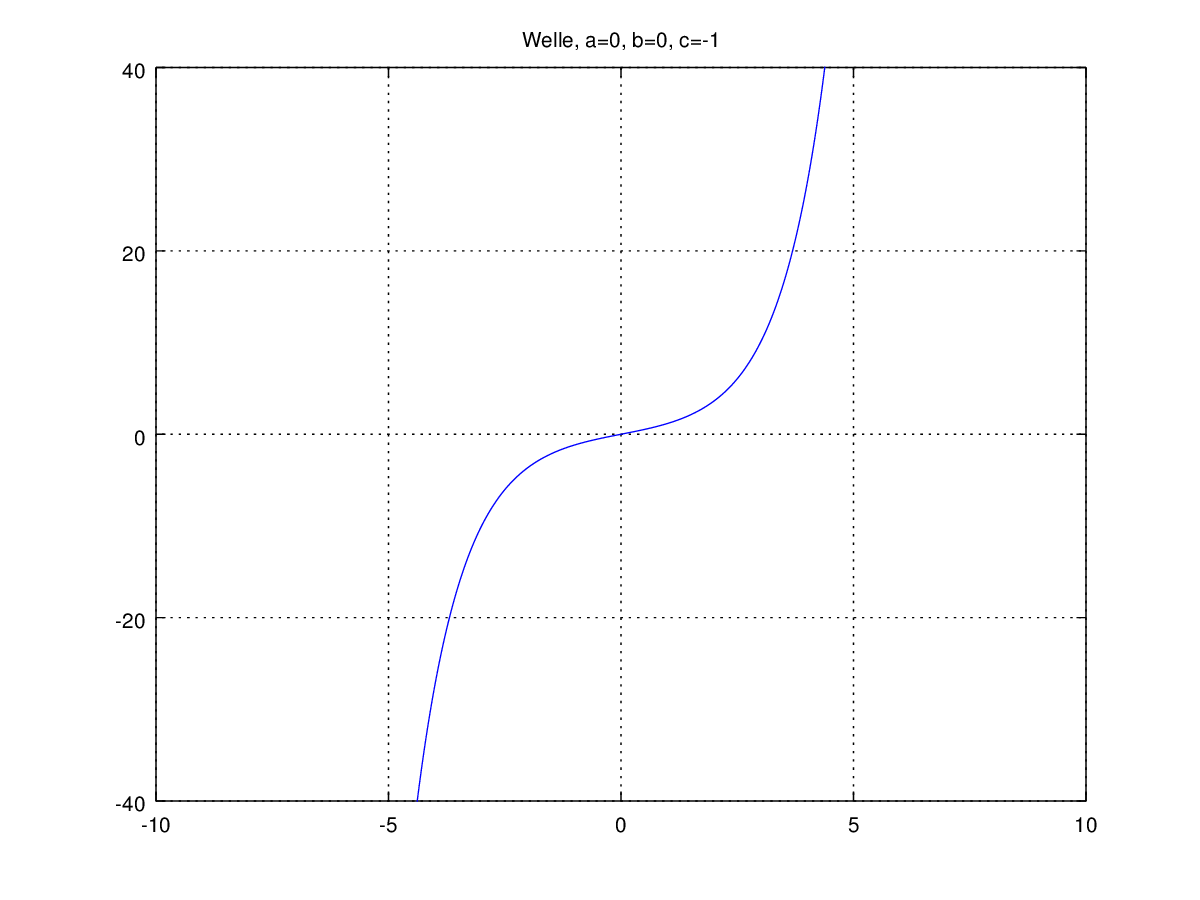
\includegraphics[scale=0.35]{./wellen/images/basicfunctions/sinh.png}
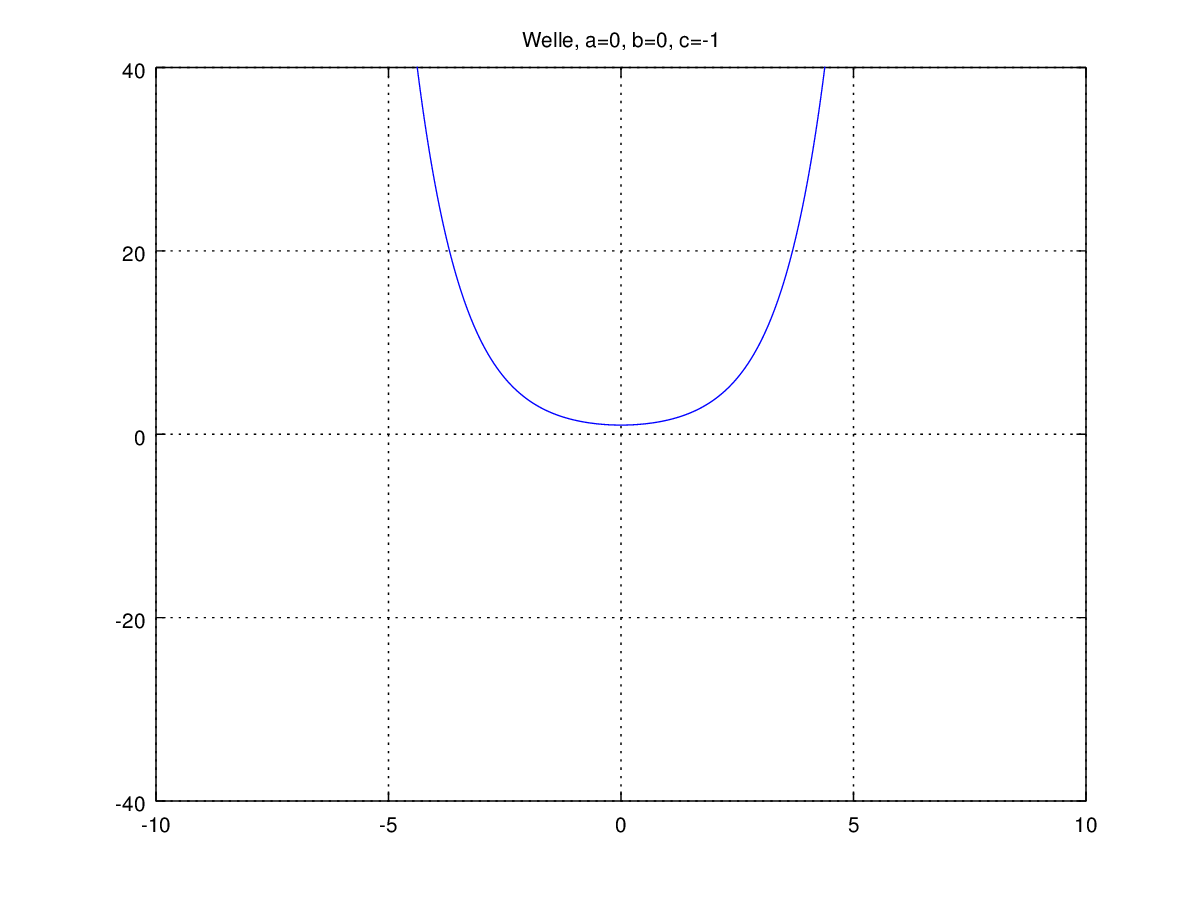
\includegraphics[scale=0.35]{./wellen/images/basicfunctions/cosh.png}

\subsection{Parabelformen}
\label{subsec:wellen:parabelformen}

Wenn nur $c$ angepasst wird erhalten wir:

\noindent
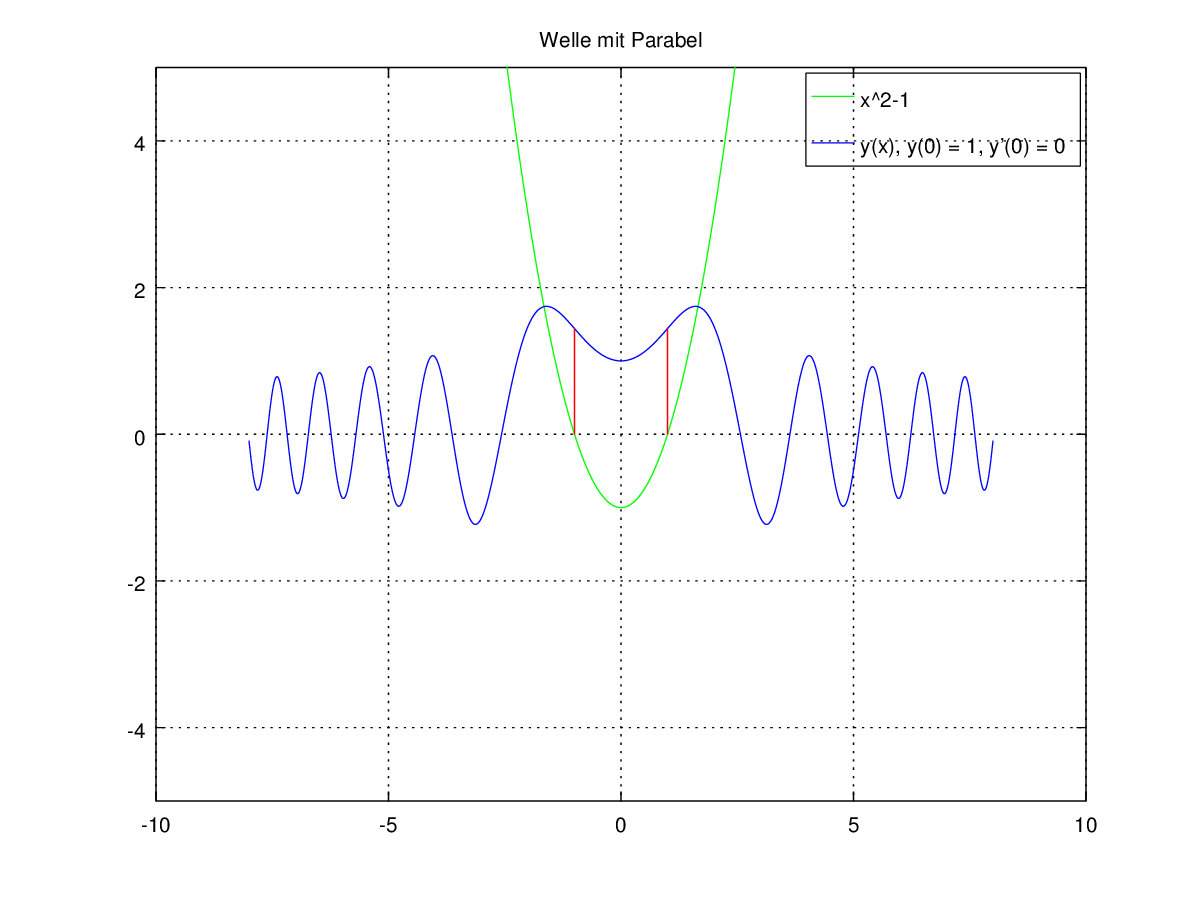
\includegraphics[scale=0.35]{./wellen/images/varc/cneg1.png}
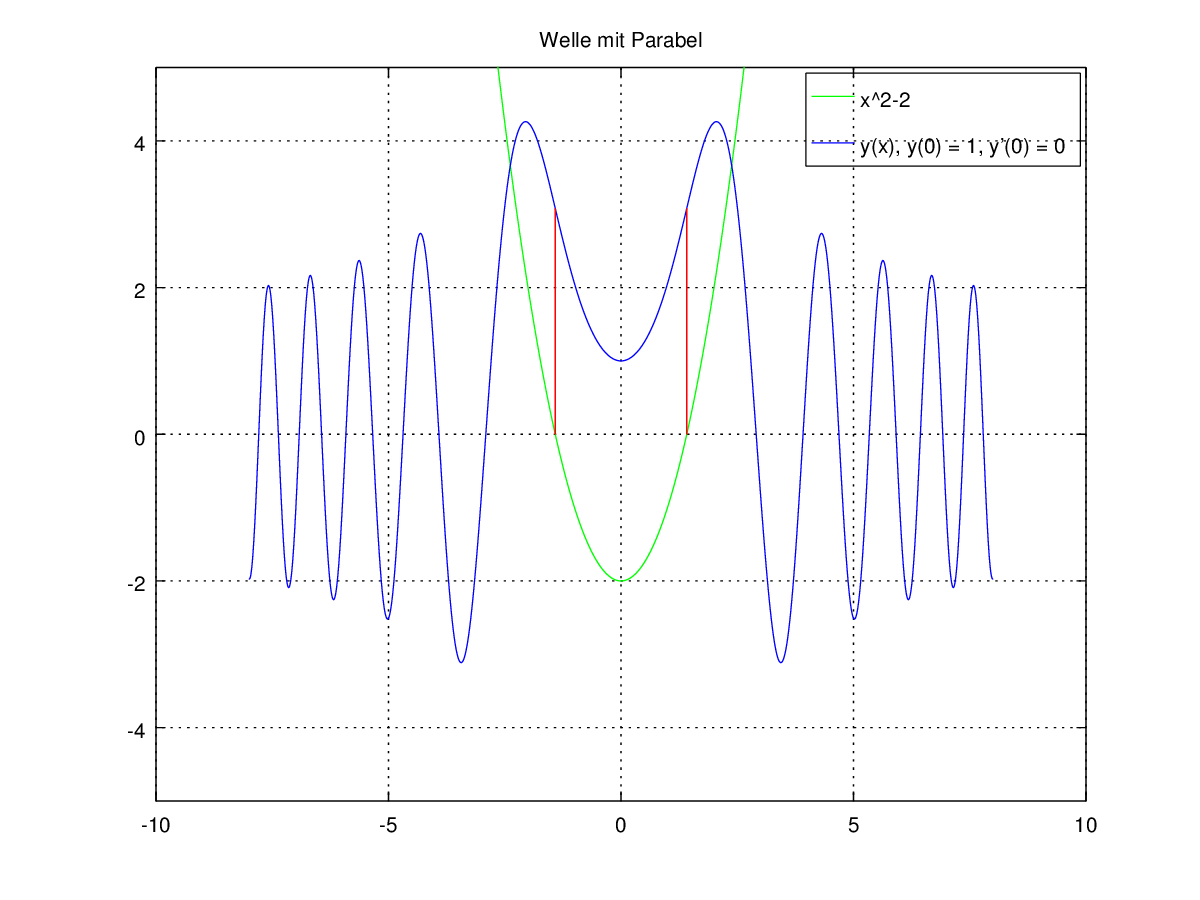
\includegraphics[scale=0.35]{./wellen/images/varc/cneg2.png}

Wenn nur $a$ angepasst wird erhalten wir:

\noindent
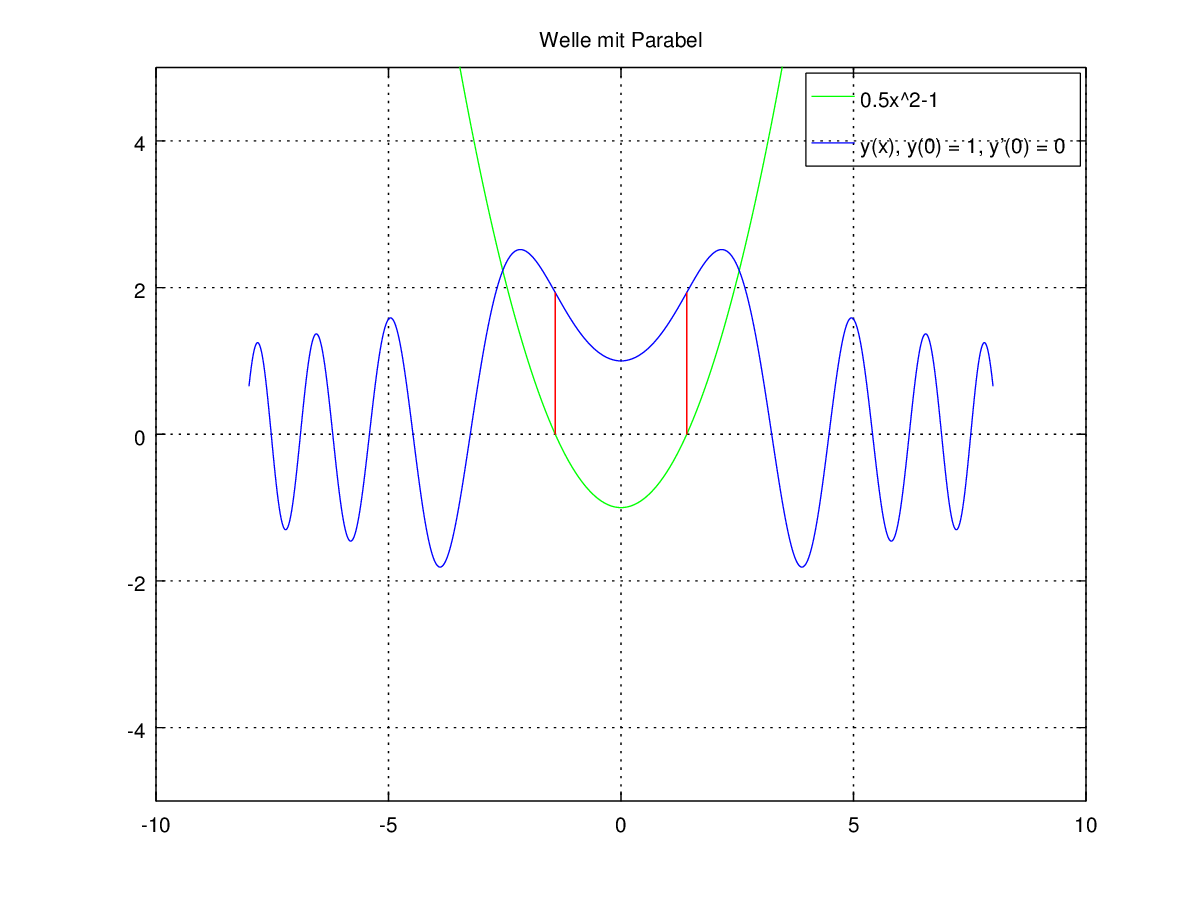
\includegraphics[scale=0.35]{./wellen/images/vara/ahalbe.png}
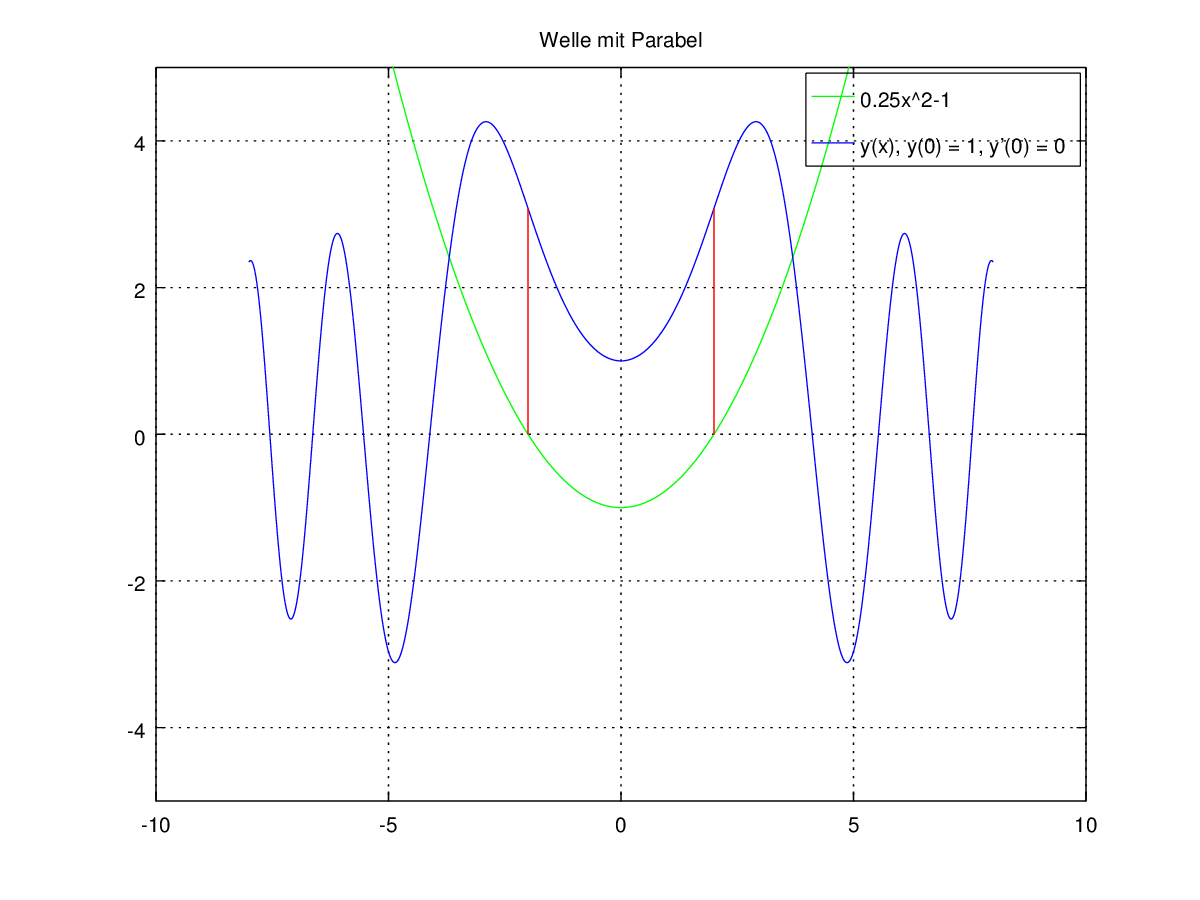
\includegraphics[scale=0.35]{./wellen/images/vara/aviertel.png}

Obwohl die Wellenformen alle "ahnlich sind, stellen wir fest, dass es bei den 
jeweiligen Nulltellen der Parabel ein gr"ossere Ver"anderung gibt.


\section{Diskussion der Wellenform}
\label{sec:wellen:DiskussionWellenform}

Wie schon in den vorhergehenden Kapiteln ersichtlich war, wechselt die Welle 
ihre Form im ``Umschlagspunkt'', welcher die Schnittpunkte der Parabel mit der 
$x$-Achse bezeichnet.


Grunds"atzlich gibt sechs untschiedliche F"alle wie die Parabel liegen kann:
\begin{itemize}
	\item Der Schnittpunkt der Parabel mit der $y$-Achse ist im negativen 
	Bereich und die Parabel nach oben ge"offnet
	\item Der Schnittpunkt der Parabel mit der $y$-Achse ist im positiven 
	Bereich und die Parabel ist nach oben ge"offnet
	\item Der Schnittpunkt der Parabel mit der $y$-Achse liegt im Nullpunkt und 
	die Parabel ist nach oben ge"offnet
	\item Der Schnittpunkt der Parabel mit der $y$-Achse ist im negativen 
	Bereich und die Parabel nach unten ge"offnet
	\item Der Schnittpunkt der Parabel mit der $y$-Achse ist im positiven 
	Bereich und die Parabel nach unten ge"offnet
	\item Der Schnittpunkt der Parabel mit der $y$-Achse liegt im Nullpunkt und 
	die Parabel ist nach unten ge"offnet
\end{itemize}

Zu Beginn wird der erste Fall betrachtet, welcher beispielsweise die Parabel 
auf der Grafik im Kapitel \ref{subsec:wellen:Variationc} beschreibt. Diese 
Parabel hat 
zwei Schnittpunkte mit der $x$-Achse und der Scheitelpunkt liegt im negativen 
$y$-Bereich. Dies bedeutet, dass alle L"osungen der Parabel von $x=0$ bis zum 
Schnittpunkt der Parabel mit der $x$-Achse negativ sind. 

Wenn nun in der Differentialgleichung f"ur die Parabel ein beliebiger negativer 
Wert eingesetzt wird, resultiert dieselbe Gleichung 
\ref{eq:wellen:LSGnegcWerte} 
wie im Kapitel \ref{subsec:wellen:Eliminierungab}. Durch das, dass die Parabel 
durch 
einen Wert ersetzt wird, ist die Aufgabenstellung die Gleiche, wie wenn man $a$ 
und $b$ eliminieren und f"ur $c$ einen negativen Wert einsetzen w"urde. In 
diesem Bereich entsteht demzufolge gem"ass Gleichung 
\ref{eq:wellen:LSGhyperbolFunktion} eine hyperbolische Funktion. Welche von den 
zwei hyperbolischen Funktionen entsteht, l"asst sich mit verschiedenen 
Anfangsbedingungen $a_0$ und $a_1$ bestimmen wie man in den folgenden Grafiken 
sieht.

GRAFIK SINH COSH

Beim Schnittpunkt der Parabel mit der $x$-Achse "andert sich das Vorzeichen der 
L"osung der Parabel und es entsteht nicht die Gleichung 
\ref{eq:wellen:LSGnegcWerte} wie oben, sondern die Gleichung 
\ref{eq:wellen:lineareDGL}, welche f"ur positive $c$-Werte aufgestellt wurde. 

Daraus wird ersichtlich, dass sich ab diesem Punkt eine L"osung einstellt, 
welche aus einer "Uberlagerung von $\sin$ und $\cos$ ist. Daraus entsteht die 
regelm"assige, kontinuierliche Schwingung. 


Bei all den anderen F"allen kann das Gleiche beobachtet werden. Bei der Parabel 
die nach oben ge"offnet ist, passiert genau das Umgekehrte. Im Innenbereich der 
Parabel entsteht eine Schwingung und sobald die Parabel die $x$-Achse schneidet 
wandelt sich die Schwingung in eine hyperbolische Funktion um. 4

Bei den Parabeln, die die $x$-Achse im Nullpunkt ber"uhren entsteht nur eine 
Schwingung, respektive nur eine hyperbolische Funktion, je nach Wert von a, 
welcher angibt, ob die Parabel nach oben oder nach unten ge"offnet ist. 
Dasselbe geschieht auch, wenn die Parabel die $x$-Achse gar nicht schneidet. 

\section{Stolpersteine}
\rhead{Stolpersteine}
Bei der Berechnung der Welle mittels Potenzreihen gibt es mehrere Dinge, die 
beachtet werden m"ussen. Von besonderer Bedeutung sind die Genauigkeit der 
L"osungen f"ur die jeweiligen $x$, sowie die Zeit, welche f"ur die 
Berechnung ben"otigt wird.

\subsubsection{Genauigkeit}
\index{Rechengenauigkeit}%
\index{Genauigkeit}%
Gem"ass
\begin{equation*}
	y(x) = \sum_{k=0}^{\textcolor{red}{\infty}}a_kx^k
\end{equation*}
m"usste man f"ur jedes $x$ eine unendliche Anzahl Additionen ausf"uhren, was 
bedeutet, dass die Berechnung f"ur ein einzelnes $x$ unendlich lange 
dauert. Folglich muss man die maximale Anzahl $k$ einschr"anken:
\begin{equation*}
	y(x) = \sum_{k=0}^{\textcolor{red}{k_{\text{max}}}}a_kx^k.
\end{equation*}
Das hat aber weitreichende Folgen: So werden je nach $k_{\text{max}}$ fr"uher 
oder sp"ater die L"osungswerte gegen $+\infty$ oder $-\infty$ gehen, was daran 
liegt, dass der Term $x^k$ einer endlichen Reihe gegen"uber den $a_k$ zu 
dominieren beginnen wird.

\begin{figure}
	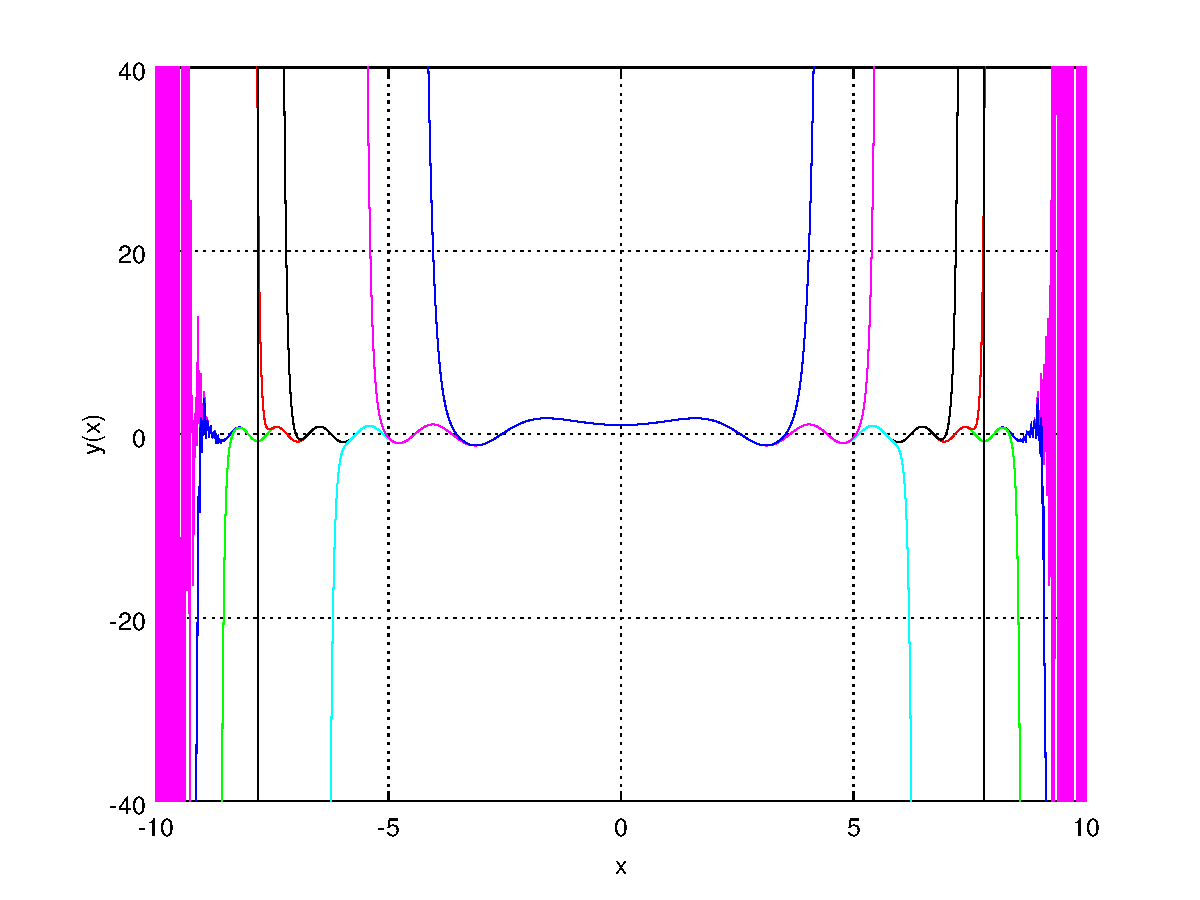
\includegraphics[width=1\hsize]{./wellen/images/kmax/kmax.pdf}
	\caption{Auswirkung $k_{\text{max}} \in [30,240]$ mit Schrittl"ange 30 auf 
	die Wellenform.}
	\label{fig:wellen:variablekmax}
\end{figure}

Die Abbildung~\ref{fig:wellen:variablekmax} zeigt auf, wie sich die L"osung 
der Titelgleichung mit verschiedenen $k_{\text{max}}$ entwickelt. Es ist leicht 
zu erkennen, dass mit gr"osser werdenden $k$ auch der Punkt, an dem $x^k$ 
dominiert, sich weiter vom Entwicklungspunkt entfernt. Es taucht noch ein 
weiteres Ph"anomen auf: Da die Werte von $a_k$ immer kleiner werden und die von 
$x^k$ immer gr"osser, kommt der Rechner an seine Grenzen und beginnt 
unbrauchbare Resultate zu liefern. Diese Ungenauigkeit ist durch die bin"are 
Darstellung von Dezimalzahlen und den Limitierungen der verschiedenen 
Datentypen wie \texttt{double} oder \texttt{float} in einem Rechnersystem 
gegeben. Diese Schwierigkeiten beschr"anken sich nicht nur auf die in diesem 
Kapitel besprochenen Probleme, sondern sind inh"arent zu allen 
Berechnungsaufgaben die mit Computern ausgef"uhrt werden.

\subsubsection{Berechnungszeit}
\index{Berechnungszeit}%

\begin{algorithm}
	\floatname{algorithm}{Pseudocode}
	\begin{algorithmic}[1]
		\State $x \gets x_{\text{min}}$
		\For{$x \le x_{\text{max}}$}
			\State $a_{-2} \gets 0$
			\State $a_{-1} \gets 0$
			\State $a_0 \gets y(0)$
			\State $a_1 \gets y'(0)$
			\State $s_{\text{series}} \gets a_0 + a_1x$
			\State $k \gets 2$
			\For{$k \le k_{\text{max}}$}
				\State $a_k \gets -\cfrac{1}{k(k-1)}			
				(aa_{k-4}+ba_{k-3}+ca_{k-2})$
				\State $s_{\text{series}} \gets s_{\text{series}} + a_k x^k$
				\State $k \gets k + 1$
			\EndFor
			\State $x \gets x + x_{\text{step}}$
		\EndFor
	\end{algorithmic}
	\caption{Wellen Potenzreihenberechnung} 
	\label{alg:wellen:potenzreihenrechnung}
\end{algorithm}

Die Berechnung von Potenzreihenl"osungen im Intervall
$[x_{\text{min}},x_{\text{max}}]$ kann "ausserst lange dauern. Auch hier muss 
die Anzahl Berechnungen, in diesem Fall die Aufl"osung des Plots, 
eingeschr"ankt werden. Eine genauere Absch"atzung kann mit Hilfe des 
Pseudocodes \ref{alg:wellen:potenzreihenrechnung} gemacht werden. Der 
Algorithmus hat eine Laufzeit von
\begin{equation*}
	O
	\left(
		k_{\text{max}}\frac{x_{\text{max}}-x_{\text{min}}}{x_{\text{step}}}
	\right).
\end{equation*}
Da einzig vier Speicherpl"atze f"ur $a_{-2}$ bis $a_1$ ben"otigt werden, hat 
dieser Algorithmus einen Speicherverbrauch von $O(1)$.
\index{Speicheraufwand}%



\begin{algorithm}
	\floatname{algorithm}{Pseudocode}
	\begin{algorithmic}[1]
		\State $a_{-2} \gets 0$
		\State $a_{-1} \gets 0$
		\State $a_0 \gets y(0)$
		\State $a_1 \gets y'(0)$
		\State $k \gets 2$
		\For{$k \le k_{\text{max}}$}
		\State $a_k \gets -\cfrac{1}{k(k-1)} (aa_{k-4}+ba_{k-3}+ca_{k-2})$
		\State $k \gets k + 1$
		\EndFor
		\State $x \gets x_{\text{min}}$
		\For{$x \le x_{\text{max}}$}
		\State $k \gets 2$
		\State $s_{\text{pot}} \gets a_0 + a_1x$
		\For{$k \le k_{\text{max}}$}
		\State $s_{\text{pot}} \gets s_{\text{pot}} + a_k x^k$
		\State $k \gets k + 1$
		\EndFor
		\State $x \gets x + x_{\text{step}}$
		\EndFor
	\end{algorithmic}
	\caption{Wellen Potenzreihenberechnung (Alternative)}
	\label{alg:wellen:potenzreihenrechnungalt}
\end{algorithm}

Nat"urlich kann man die $a_k$ auch bereits vorg"angig berrechnen. Was uns zum 
Pseudocode \ref{alg:wellen:potenzreihenrechnungalt} f"uhrt. Dieser 
alternative Algorithmus hat eine Laufzeit von
\begin{equation*}
	\mathcal{O}
	\left(k_{\text{max}} + 
		k_{\text{max}}\frac{x_{\text{max}}-x_{\text{min}}}{x_{\text{step}}}
	\right)
	=
	\mathcal{O}
	\left(
		k_{\text{max}}
		\left(
			1+\frac{x_{\text{max}}-x_{\text{min}}}{x_{\text{step}}}
		\right)
	\right),
\end{equation*}
und einen Speicherverbrauch von
\begin{equation*}
	\mathcal{O}
	\left(
		k_{\text{max}}
	\right).
\end{equation*}

Mit dieser Diskussion verlassen wir das parabolische Profil und betrachten 
allgemeinere Aspekte wie Stolpersteine bei der Ausf"uhrung solcher Berechnungen 
oder die verallgemeinerte L"osung von Differentialgleichungen 
dieser Art mit einem Profil der Form
\begin{equation*}
p(x) = \sum_{i=0}^{n} \lambda_i x^i.
\end{equation*}


\section{Allgemeines Polynom}

\begin{equation}
	y''+\sum_{i=0}^{n}\lambda_ix^i y=0, \quad n \ge 0
	\label{wellen:allgemeinesproblem}
\end{equation}

Aufgrund der bisherigen Beobachtungen ist es nun m"oglich, eine 
allgemein geltende Potenzreihenl"osung f"ur diese Art Differentialgleichungen 
zu erstellen.

Hierzu wird die anf"angliche Parabel $ax^2 + bx + c$ mit dem allgemeinen Polynom

\begin{equation*}
	\lambda_nx^n + \lambda_{n-1}x^{n-1} + \lambda_{n-2}x^{n-2} + \dotsb + 
	\lambda_2x^2 + \lambda_1x + \lambda_0 = \sum_{i=0}^{n}\lambda_ix^i, \quad n 
	\ge 0
\end{equation*}
ersetzt.

Bei der neuen Problemstellung handelt es sich immernoch um eine 
Differentialgleichungen zweiter Ordnung. Es bleibt also eine Abh"angigkeit von 
mindestens zwei zwischen den verschiedenen $a_k$. Zus"atzlich erh"oht sich 
diese jeweils um den Polynomkoeffizientenindex. Daraus folgt nun

\begin{equation*}
	a_k = -\frac{1}{k(k-1)}\sum_{i=0}^{n}a_{k-2-i)}\lambda_i, \quad n \ge 0, 
	a_{k-2-i < 0} =  0.
\end{equation*}
f"ur ein Polynom $n$-ten Grades.

Die Potenzreihenl"osung f"ur \ref{wellen:allgemeinesproblem} lautet somit:
\begin{equation}
	y(x) = a_0 + a_1x - \sum_{k=2}^{\infty}\frac{1}{k(k-1)}\sum_{i=0}^{n}
	\lambda_ia_{k-2-i}x^k, \quad n \ge 0, a_{k < 0} = 0
	\label{wellen:allgemeineloesung}
\end{equation}

\subsection{Schlussfolgerungen}

Mit der Formel \ref{wellen:allgemeineloesung} gibt es nun ein einfaches 
Werkzeug mit dem man allein durch Einsetzen die Potenzreihenl"osung f"ur 
diese Art von Differentialgleichungen erh"alt.

Sie erlaubt es uns aber auch noch weitere Schl"usse zu ziehen. So kann man 
nun direkt aus der Form der L"osung des gegebenen Polynoms ablesen, wie sich 
die Differentialgleichung verhalten wird. Soll heissen, positive L"osungen 
f"uhren zu einer Wellenform, die $\sin$ und $\cos$ enthalten. Negative 
L"osungen liefern hingegen eine Kombination aus $\sinh$ und $\cosh$.

\subsection{Beispiel: $n = 1$, Airy-Differentialgleichung}
Die bereits bekannte Airy-Differentialgleichung
\begin{align*}
	y''-xy = 0
\end{align*}
ergibt nun in die allgemeine L"osungsformel \ref{wellen:allgemeineloesung} 
eingesetzt:

\begin{equation*}
\begin{split}
	y(x) &= a_0+a_1x-\sum_{k=2}^{\infty} \frac{1}{k(k-1)} ((-1) a_{k-2-1} + 0 
	a_{k-2-0}) x^k
	\\
	&= a_0+a_1x+\sum_{k=2}^{\infty} \frac{1}{k(k-1)} a_{k-3} x^k,
	\qquad a_{k < 0} = 0
\end{split}
\end{equation*}

Graphisch betrachtet werden die genannten Konsequenzen deutlich erkennbar:

\begin{center}
	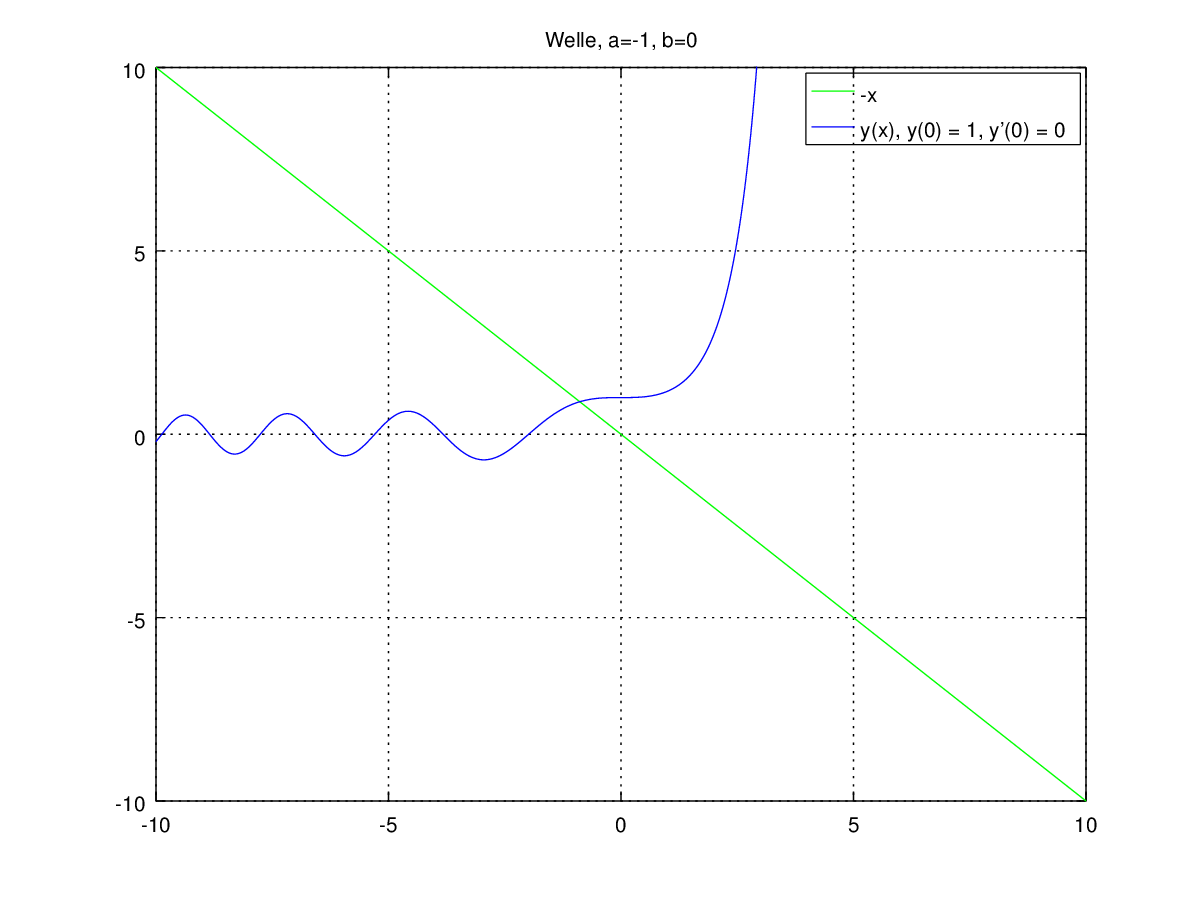
\includegraphics[scale=0.65]{./wellen/images/allgemein/n1.png}
\end{center}

\subsection{Beispiel: $n = 4$}

Auch ein Polynom 4-ten Grades stellt kein Problem dar. Die 
Differentialgleichung:

\begin{equation*}
	y''+(ax^4+bx^3+cx^2+dx+e)y = 0
\end{equation*}
ergibt nach dem Einsetzen:

\begin{align*}
	y(x) &= a_0+a_1x-\sum_{k=2}^{\infty} \frac{1}{k(k-1)} (aa_{k-2-4} + 
	ba_{k-2-3} + ca_{k-2-2} + da_{k-2-1} +ea_{k-2-0})x^k
	\\
	&= a_0+a_1x-\sum_{k=2}^{\infty} \frac{1}{k(k-1)} (aa_{k-6} + ba_{k-5} + 
	ca_{k-4} + da_{k-3} +ea_{k-2})x^k, \qquad a_{k<0} = 0
\end{align*}

Auch hier kann man graphisch die "Uberg"ange zwischen $\sin$ und $\cos$ bei 
positiven und $\sinh$ und $\cosh$ bei negativen Polynoml"osungen klar erkennen.

\begin{center}
	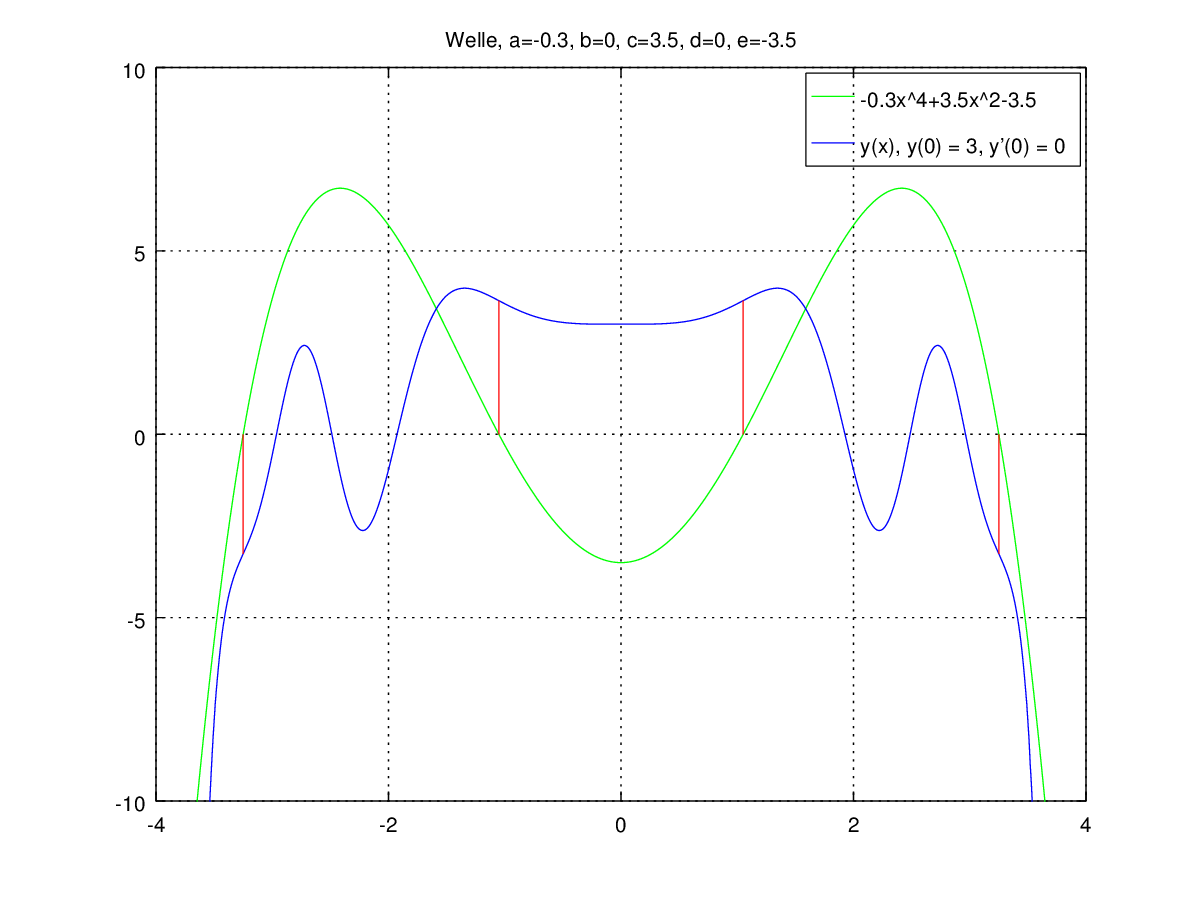
\includegraphics[scale=0.65]{./wellen/images/allgemein/n4.png}
\end{center}

\printbibliography[heading=subbibliography]
\end{refsection}